\documentclass[aps,prb,reprint,showpacs,floatfix,superscriptaddress, onecolumn, nofootinbib, 9pt]{revtex4-2}

\usepackage{amsmath,amsthm,amssymb}
\usepackage{graphicx}% Include figure files
\usepackage{dcolumn}% Align table columns on decimal point
\usepackage{bm}% bold math
\usepackage{color}
\usepackage{epsfig}
\usepackage{multirow}
\usepackage{mathrsfs}
\usepackage{hyperref}
\usepackage{cleveref}
\usepackage{epstopdf}
\usepackage{subfigure}
\usepackage{autobreak}
\usepackage{todonotes}
\usepackage{physics}
\usepackage{bbm}



\usepackage[absolute,overlay]{textpos}

%Macros for mathematical notations

\newcommand{\V}[1]{\boldsymbol{#1}} %# vector
\newcommand{\M}[1]{\boldsymbol{#1}} %# matrix
\newcommand{\Set}[1]{\mathbb{#1}} %# set
\newcommand{\D}[1]{\Delta#1} %# \D{t} for time step size
\renewcommand{\d}[1]{\delta#1} %# \d{t} for small increment
\newcommand{\av}[1]{\left\langle #1\right\rangle } %take average

\newcommand{\sM}[1]{\M{\mathcal{#1}}} %matrix in mathcal font
\newcommand{\dprime}{\prime\prime} % double prime
%\global\long\def\i{\iota}
%\renewcommand{\i}{\iota} %i for imaginary unit
%\renewcommand{\i}{\mathsf i} %i for imaginary unit
\newcommand{\follows}{\quad\Rightarrow\quad} %=>
\newcommand{\eqd}{\overset{d}{=}} %=^d
\newcommand{\spe}[1]{\mathscr{#1}}  %important quantities in mathscr font
\newcommand{\eps}{\epsilon}

\newcommand{\response}[1]{{\color{blue}#1}} % for authors' response


\begin{document}
	\preprint{Preprint}
	
	\title{Response to Referee Comments for Manuscript BH14505}
	\author{Analabha Roy}
	\date{\today}
	
	\maketitle
	
	\vspace{1em}
	
	\noindent \textbf{Response to First Referee}
	
	\begin{enumerate}
		\item The referee says, ``\textit{A brief comparison of this work to other works on periodically driven LMG models and DMBL is needed somewhere in the introductory sections to state what is the significance and novelty of this work. }"\\
		
		\response{
			We thank the referee for this suggestion. In earlier work on periodically driven LMG models,
			the focus was on determining the onset of DMBL by looking at expectation values of local
			observable(s) . Standard quantities that have been observed include magnetization, heating rate, and fidelity susceptibility. The observables were calculated by running simulations over an long duration, and localization was inferred from their dynamics over long but ultimately finite times.
			
			The novelty of our paper lies in the search for DMBL in the Floquet qusaistationary states of the LMG model themselves, rather than in the observable dynamics. Localization in the Floquet modes can be deduced from the values of their Inverse Participation Ratio, which distinguishes between a fully localized state and a thermal state of the system. IPR ranges from scaling inversely with the Hilbert space dimension (a fully distributed or thermal state) to unity (a fully localized state). Our view is that this is a better indicator of localization, as it is valid for infinite times, as opposed to observable dynamics, where very long time effects are inconclusive. We have updated our introduction to elaborate on this.
		


}
		\item The referee says, ``\textit{On page 3, the Floquet eigenstate Thermalization hypothesis is stated without references. }".\\
		
		\response{
			We thank the referee for pointing out this mistake. In the manuscript, we have provided proper references to FETH.
		}
		
		\item The referee says, "\textit{On page 4, after illustrating the resonances in the analytically solvable TFIM model, the authors claim, “This phenomenon is highly general and can be readily adapted to non-integrable systems”. I disagree with the statement, and clear references, if any, need to be cited to back up this statement. The manipulations made for TFIM are fine-tuned to this integrable system, and they break down the moment any integrability-breaking term is introduced. For example, if I add a longitudinal field sigma-x to the TFIM, I do not see how to adapt the procedure. }"\\
		\textbf{Math needs correcting}
		\response{ We would like to thank the referee for this comment. We acknowledge that there may have been a lack of clarity regarding this matter in the manuscript. We have revised some of the content in the manuscript to elaborate on this. A short summary follows:
			
			We utilized the RWA on the Hamiltonian following the unitary transformation to investigate localization in TFIM. Adding a longitudinal field $\sigma^x$ to the original TFIM Hamiltonian destroys the integrability of the model. However, it does not cause the math to break down completely.  Adding a symmetry-breaking field $\sigma^x$ to the driven TFIM yields 
			\begin{equation}
				\hat{\mathcal{H}}(t) =\frac{1}{2}\left[\sum_{i} J \hat{\sigma}_{i}^{x} \hat{\sigma}_{i+1}^{x}+\sum_{i} \hat{\sigma}_{i}^{x}+h \cos (\omega t) \sum_{i} \hat{\sigma}_{i}^{z}\right]
			\end{equation}
			In order to move to the rotating frame, the transformation operator to be applied is $\displaystyle \hat{U}(t)$ is, $\hat{U}(t)=\prod_{i} \exp \left(-i \frac{h}{2 \omega} \sin (\omega t) \hat{\sigma}_{i}^{z}\right)$. Thus,
			\begin{align}
				\tilde{\mathcal{H}}(t)= & \frac{1}{2} \exp \left(i \frac{h}{2 \omega} \sin (\omega t) \sum_{i} \hat{\sigma}_{i}^{z}\right)\left(\sum_{i} J \hat{\sigma}_{i}^{x} \hat{\sigma}_{i+1}^{x}+\sum_{i} \hat{\sigma}_{i}^{x}\right) \exp \left(-i \frac{h}{2 \omega} \sin (\omega t) \sum_i\hat{\sigma}_{i}^{z}\right) \nonumber\\
				= & \underbrace{\frac{1}{2} \exp \left(i \frac{h}{2 \omega} \sin (\omega t) \sum_{i} \hat{\sigma}_{i}^{z}\right)\left(\sum_{i} J \hat{\sigma}_{i}^{x} \hat{\sigma}_{i+1}^{x}\right) \exp \left(-i \frac{h}{2 \omega} \sin (\omega t) \sum_i\hat{\sigma}_{i}^{z}\right)}_{\mathrm{A}} \nonumber\\
				& +\underbrace{\frac{1}{2} \exp \left(i \frac{h}{2 \omega} \sin (\omega t) \sum_{i} \hat{\sigma}_{i}^{z}\right)\left(\sum_{i} \hat{\sigma}_{i}^{x}\right) \exp \left(-i \frac{h}{2 \omega} \sin (\omega t) \sum_i\hat{\sigma}_{i}^{z}\right)}_{\mathrm{B}}.
				\label{eq:rotated:hamilt}
			\end{align}
			where we have split the result into two terms labeled $A$ and $B$. We now apply the RWA to both terms separately. First, let us define $\eta=\frac{h}{2 \omega} \sin (\omega t)$. The first term becomes
			\begin{align}
				A &= \prod_i \exp\left(i\eta\hat{\sigma}^z_i\right)\left(\sum_{i} J \hat{\sigma}_{i}^{x} \hat{\sigma}_{i+1}^{x}\right)\exp\left(-i\eta\hat{\sigma}^z_i\right)\nonumber\\
				&= \sum_i J \exp(i\eta\hat{\sigma}^z_i)\exp(i\eta\hat{\sigma}^z_{i+1})\left( \hat{\sigma}_{i}^{x} \hat{\sigma}_{i+1}^{x}\right)\exp(-i\eta\hat{\sigma}^z_i)\exp(-i\eta\hat{\sigma}^z_{i+1})\nonumber\\
				&= J\sum_{i} \hat{\sigma}_{i}^{x} \hat{\sigma}_{i+1}^{x}\exp(-2i\eta\hat{\sigma}^z_i)\exp(-2i\eta\hat{\sigma}^z_{i+1})
				\label{eq:hmov}
			\end{align}
			Now, we use the expression, $\displaystyle e^{ia(\hat{n}\cdot \vec{\sigma})} = \mathbbm{1} \cos(a) + i (\hat{n}\cdot \vec{\sigma})\sin(a)$ on the exponents in the RHS above. This yields
			\begin{align}
				\exp\left(-2i\eta\hat{\sigma}^z_i\right)\exp\left(-2i\eta\hat{\sigma}^z_{i+1}\right)
				=& \Big[\mathbbm{1} \cos(2\eta) - i \hat{\sigma}^z_i\sin(2\eta)\Big]\Big[\mathbbm{1} \cos(2\eta) - i \hat{\sigma}^z_{i+1}\sin(2\eta)\Big]\nonumber\\
				=& \mathbbm{1} \cos^2(2\eta) - \hat{\sigma}^z_i\hat{\sigma}^z_{i+1}\sin^2(2\eta) -\frac{i}{2} \left(\hat{\sigma}^z_i+ \hat{\sigma}^z_{i+1}\right)\sin(4\eta)
				\label{eq:op}
			\end{align}
			Next, we note the trigonometric identities
			\begin{align}
				\cos^2(2\eta) =& \frac12\big[1+\cos(4\eta)\big]=\frac12\big[\cos^2(4\eta)+ \sin^2(4\eta)+\cos(4\eta)\big]\nonumber\\
				\sin^2(2\eta) =& \frac12\big[1-\cos(4\eta)\big]=\frac12\big[\cos^2(4\eta)+ \sin^2(4\eta)-\cos(4\eta)\big]
				\label{eq:cossin}
			\end{align}
			The Jacobi Anger expansion yields
			\begin{align}
				\cos (4 \eta)&=\cos \left(\frac{2 h}{\omega} \sin (\omega t)\right)=\mathcal{J}_{0}\left(\frac{2 h}{\omega}\right)+2 \sum_{n=1}^{\infty}(-1)^{n} \mathcal{J}_{2 n}\left(\frac{2 h}{\omega}\right) \cos (2 n \omega t),\label{eq:jacang1} \\
				\sin (4 \eta)&=\sin \left(\frac{2 h}{\omega} \sin (\omega t)\right)=-2 \sum_{n=1}^{\infty}(-1)^{n} \mathcal{J}_{2 n-1}\left(\frac{2 h}{\omega}\right) \cos [(2 n-1) \omega t],
				\label{eq:jacang2}
			\end{align}
			where $\mathcal{J}_{n}$ is the Bessel function of $n^{th}$ order. Now, in the RWA, we can neglect the terms in this expansion that oscillate at a faster rate than the drive frequency $\omega$. This yields $ \cos (4 \eta) \approx\mathcal{J}_{0}\displaystyle\left(\frac{2 h}{\omega}\right)$, and $\sin(4\eta)\approx 0$. Substituting in Eq.~\ref{eq:cossin} yields further approximations
			\begin{align}
				\cos^2(2\eta) \simeq& \frac12\Bigg[\left\{\mathcal{J}_0\left(\frac{2h}{\omega}\right)\right\}^2 + \mathcal{J}_0\left(\frac{2h}{\omega}\right)\Bigg]=\frac12 \mathcal{J}_0\left(\frac{2h}{\omega}\right)\Bigg[1+ \mathcal{J}_0\left(\frac{2h}{\omega}\right)\Bigg]\nonumber\\
				\sin^2(2\eta) \simeq& \frac12\Bigg[\left\{\mathcal{J}_0\left(\frac{2h}{\omega}\right)\right\}^2 - \mathcal{J}_0\left(\frac{2h}{\omega}\right)\Bigg]=\frac12 \mathcal{J}_0\left(\frac{2h}{\omega}\right)\Bigg[1- \mathcal{J}_0\left(\frac{2h}{\omega}\right)\Bigg]
			\end{align}
			\todo{Revisit the math here}
			Substituting these into Eq.~\ref{eq:op} yields
			\begin{equation}
				\exp\left(-2i\eta\hat{\sigma}^z_i\right)\exp\left(-2i\eta\hat{\sigma}^z_{i+1}\right) \approx \frac12 \mathcal{J}_0\left(\frac{2h}{\omega}\right)\Bigg[\left\{1+ \mathcal{J}_0\left(\frac{2h}{\omega}\right)\right\} - \hat{\sigma}^z_i\hat{\sigma}^z_{i+1}\left\{1- \mathcal{J}_0\left(\frac{2h}{\omega}\right)\right\} \Bigg]
			\end{equation}
			Substituting this into  Eq.~\ref{eq:hmov} finally yields the RWA approximation for $A$,
			\begin{align}
				A^{R W A}&=\frac{J}{2} \mathcal{J}_0\left(\frac{2h}{\omega}\right)\sum_{i}\Bigg[\left\{1+ \mathcal{J}_0\left(\frac{2h}{\omega}\right)\right\} \hat{\sigma}_{i}^{x} \hat{\sigma}_{i+1}^{x} + \hat{\sigma}^y_i\hat{\sigma}^y_{i+1}\left\{1- \mathcal{J}_0\left(\frac{2h}{\omega}\right)\right\} \Bigg]
				\label{eq:hrwa1}
			\end{align}
			Next, we obtain the RWA approximation for $B$. First, we define proper angular momenta $\displaystyle S^{\mu(=x,y,z)} = \frac12\sum_i \hat{\sigma}^\mu_i$, so that we can write
			\begin{align*}
				B & =\frac{1}{2} \exp \left(i \frac{h}{2 \omega} \sin (\omega t) \sum_{i} \hat{\sigma}_{i}^{z}\right)\left(\sum_{i} \hat{\sigma}_{i}^{x}\right) \exp \left(-i \frac{h}{2 \omega} \sin (\omega t) \hat{\sigma}_{i}^{z}\right) \\
				& =\left(e^{i 2 \eta S^{z}} S^{x} e^{-i 2 \eta S^{z}}\right),
			\end{align*}
			where we have used the Baker-Campbell-haussdorff formula, together with the canonical angular momentum commutation relations. Applying the Jacobi Anger expansion again, recalling that $\eta=\frac{h}{2 \omega} \sin (\omega t)$ and taking the RWA that keeps only $n=0$'th term,
			\begin{equation}
				B^{RWA} = \left(S^{x} \cos (2 \eta)-S^{y} \sin (2 \eta)\right) \simeq \mathcal{J}_{0}\left(\frac{h}{\omega}\right) S^{x} = \mathcal{J}_{0}\left(\frac{h}{\omega}\right)\frac12\sum_i\hat{\sigma}^x_i
				\label{eq:B}
			\end{equation}
			Substituting Eqs~\ref{eq:hrwa1} and ~\ref{eq:B} as RWA approximations into Eq~\ref{eq:rotated:hamilt} yields the final RWA Hamitonian
			\begin{equation}
				\hat{\mathcal{H}}_{_{TFIM+S_{x}}}^{R W A}=\frac{J}{2} \mathcal{J}_0\left(\frac{2h}{\omega}\right)\sum_{i}\Bigg[\left\{1+ \mathcal{J}_0\left(\frac{2h}{\omega}\right)\right\} \hat{\sigma}_{i}^{x} \hat{\sigma}_{i+1}^{x} + \hat{\sigma}^y_i\hat{\sigma}^y_{i+1}\left\{1- \mathcal{J}_0\left(\frac{2h}{\omega}\right)\right\} \Bigg] +\mathcal{J}_{0}\left(\frac{h}{\omega}\right) \frac12\sum_i\hat{\sigma}^x_i
				\label{eq:tfimpsx}
			\end{equation}
			There isn't a single point in the ($h, \omega$) parameter space  where this RWA Hamiltonian vanishes, unlike the TFIM case. However, when $\mathcal{J}_0(2h/\omega)$ vanishes, the RWA Hamiltonian simply reduces to $\mathcal{J}_0(h/\omega) S^x$ and, therefore, is diagonal in the representation spanned by eigenstates of the longitudinal field. Thus, the IPR of the Floquet states, taken in this representation, will be unity. This recovers DMBL, albeit in a different representation. We can argue that the physically significant representation is the one spanned by the eigenstates of the symmetry breaking observable.}
		\item The referee says,``\textit{In the discussion of phase crossover from thermal to DMBL, increasing N in Fig 8 appears to push the regime of the local phase to a larger drive frequency. This seems to raise the same concerns associated with the stability of disorder-induced localization, as in whether one needs infinite disorder or infinite driving frequency to
			get a localization in the thermodynamic limit. Is this the case? }".
		
		\response{    	
			We thank the referee for the comment. We have extended or simulations for larger system sizes and have verified that this is, indeed, the case. Increasing $N$ pushes the crossover point further to larger values of $\omega$, thus requiring infinite frequency at infinite size. We have updated the corresponding Fig.8 with a revised version, and have reported this in section 4 par 2.
		}
		\item The referee says,``\textit{Is the heating suppressed at points where the frequency meets the resonance condition? }".
		\todo{rewrite}
		\response{
			We thank the referee for this comment. We agree with understanding of the referee. The resonance condition derived from the Rotating Wave Approximation(RWA) over the Hamiltonian of system. At resonance condition(s), it is possible to nullify the effective Hamiltonian. This results in total localization of the system. This is true for infinite times. Thus the system at resonance condition never undergo the heating.
		}
		
		\item The referee says, ``\textit{The discussion related to Fig. 9 could be improved, and it is not clear to me why the standard deviation of temporal fluctuations should vanish for thermalizing systems. }"\\
		
		\response{ We thank the referee to point out the issue. We agree to improve the discussion and rectify our results. We have revised the discussion as well as improved the corresponding Fig.(9) also.
			
			
			The Hamiltonian for LMG model,
			\begin{equation}
				\mathcal{H} = \frac{J}{2(N-1)}\sum_{i\neq j}\hat{\sigma}^z_i \hat{\sigma}^z_j + (h_0 +h_1 \cos(\omega t) \sum_i \hat{\sigma}^x_i
			\end{equation}
			In the full Hilbert space, considering the dc part ($h_0$) of the drive is very negligibly small, the time average of the Hamiltonian,
			\begin{equation*}
				\bar{H}_0 = \frac{J}{2(N-1)}\sum_{i\neq j}\hat{\sigma}^z_i \hat{\sigma}^z_j.
			\end{equation*}
			Similarly,
			\begin{equation}
				\left(\bar{H_0}\right)^2 = \frac{J^2}{4(N-1)^2}\sum_{i\neq j, k \neq l} \hat{\sigma}^z_i \hat{\sigma}^z_j \hat{\sigma}^z_k \hat{\sigma}^z_l
			\end{equation}
			
			The thermal variance at $T= \infty$ is given by $\displaystyle \sigma^2_{\infty} = \frac{\Tr[H^2_0]}{2^N}$. 
			
			\begin{figure}[h!]
				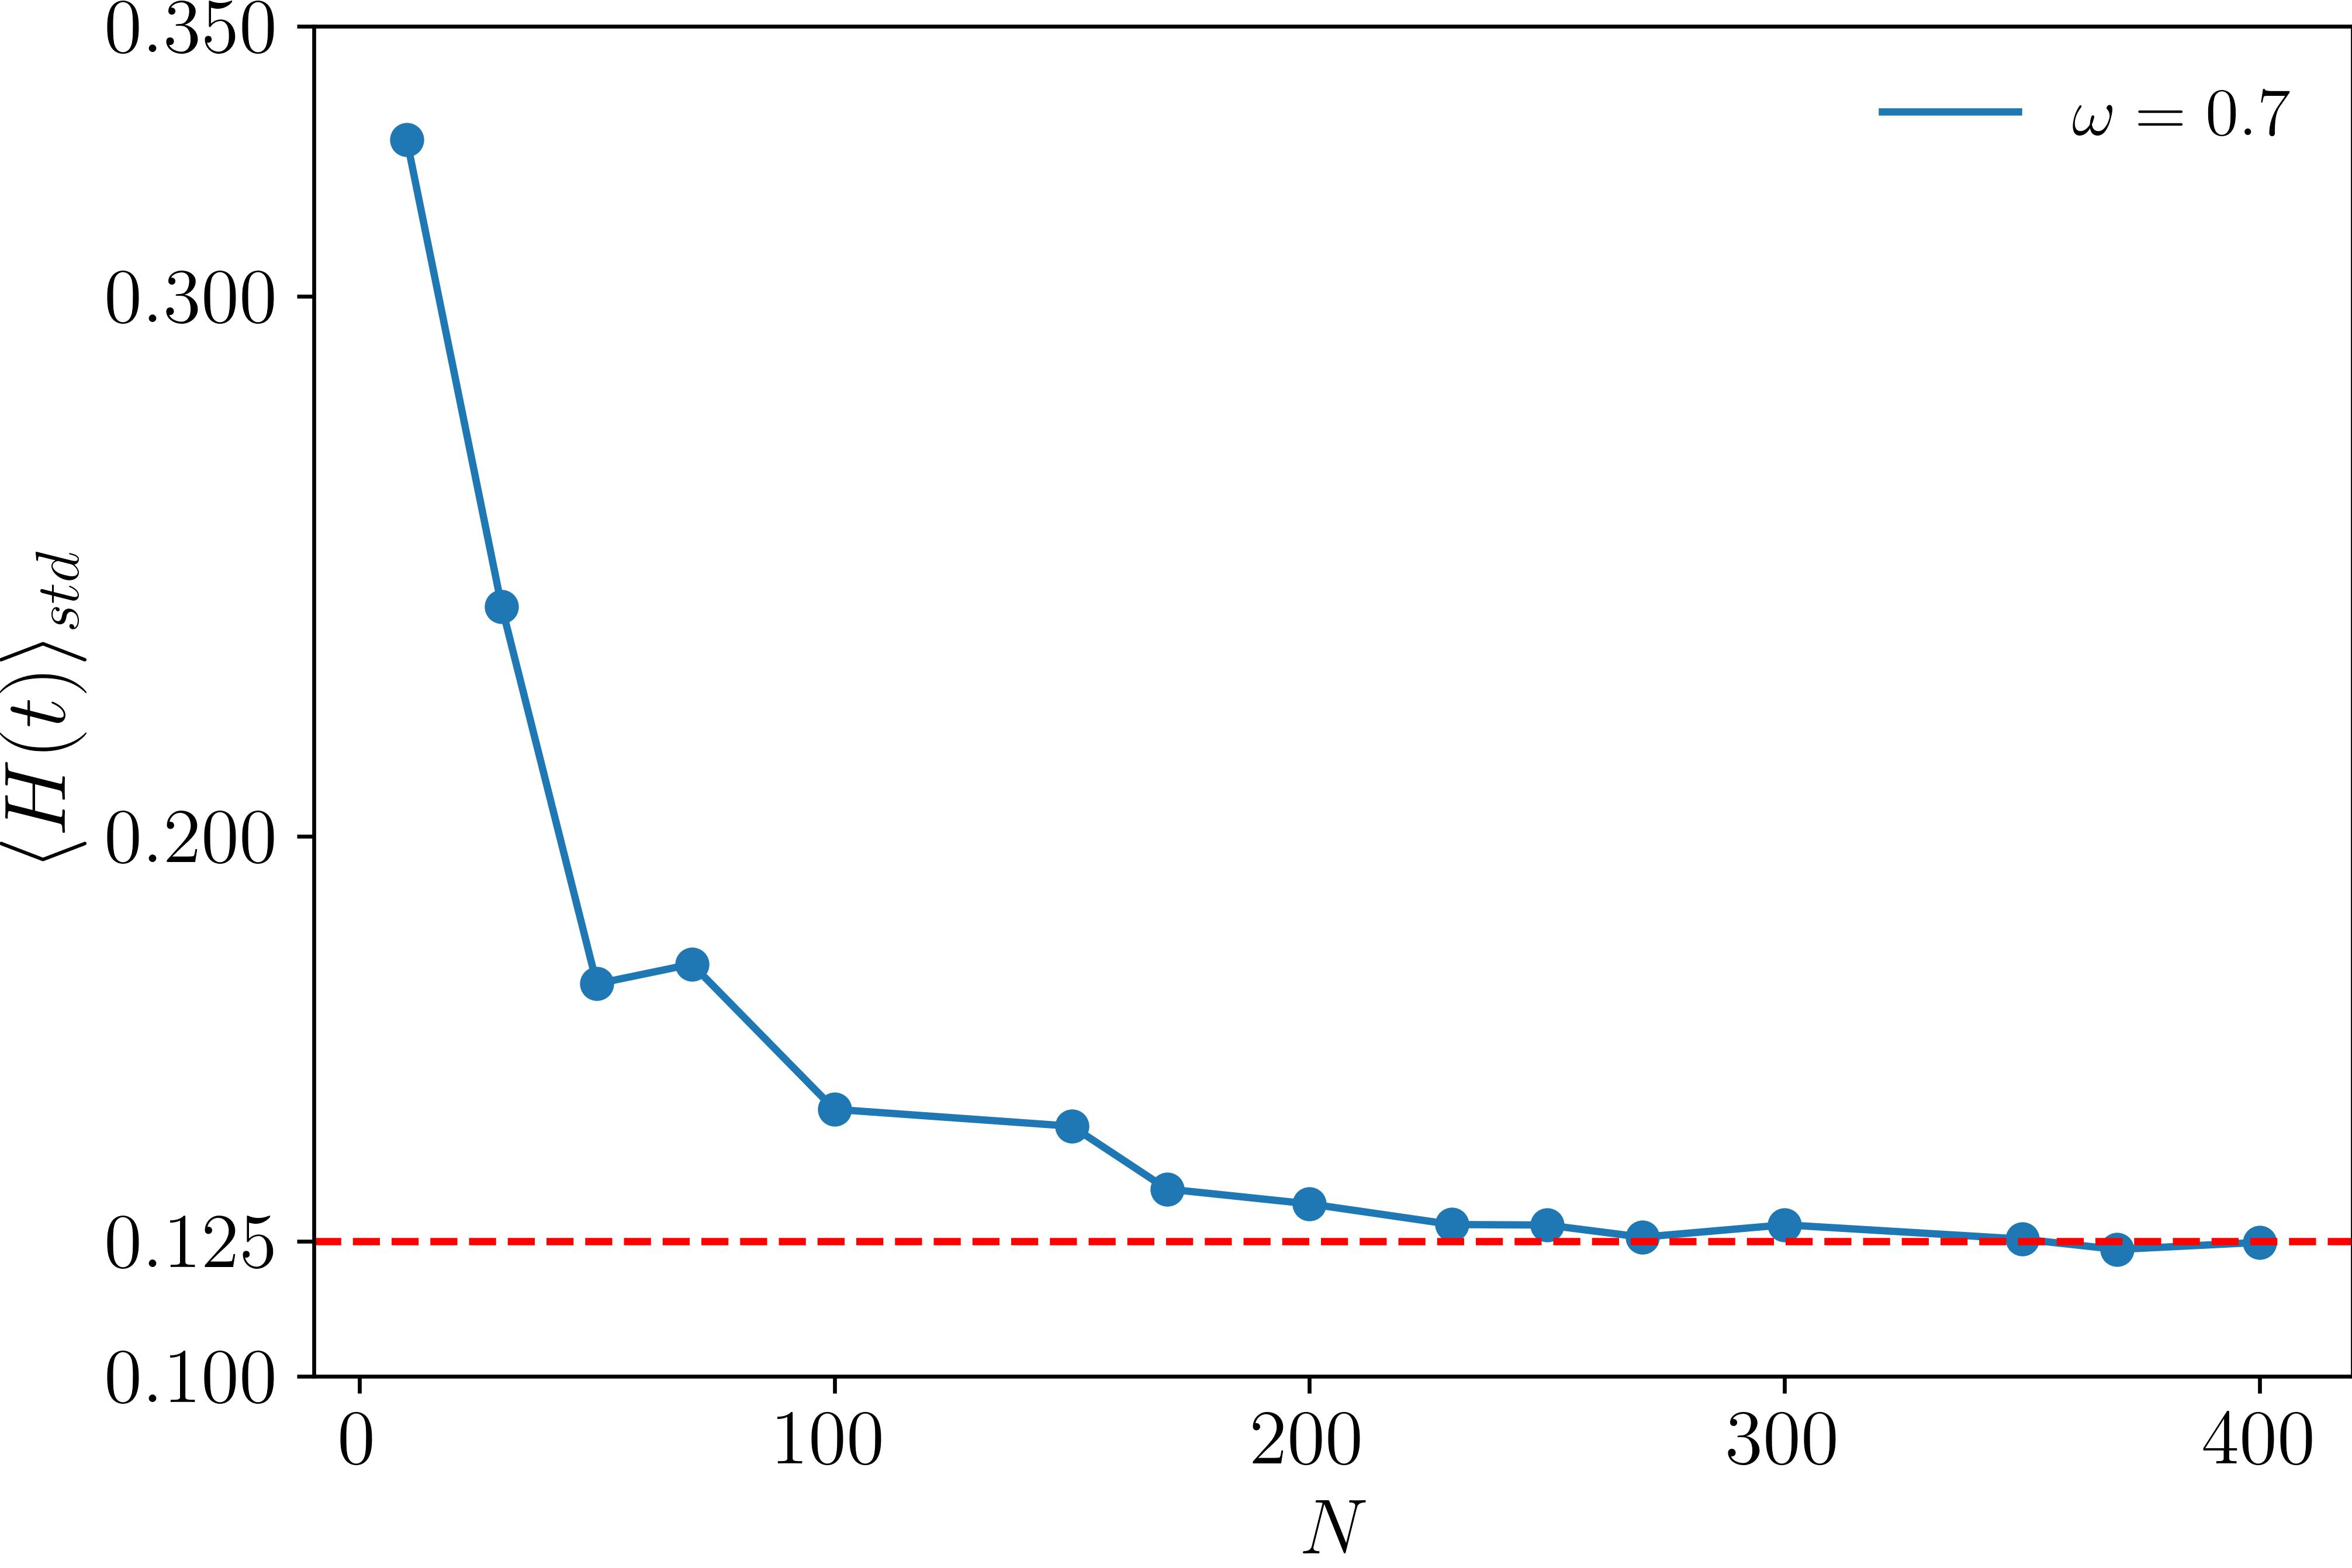
\includegraphics[width=8.5cm]{hbar_avg_std_w0.7.jpg}
				\caption{Variation of $\expval{H(t)}_{std}$ with system size(N) at small frequency $\omega=0.7$. $\expval{H(t)}_{std}$ is found to decrease as N increases and at thermodynamic limit it reaches 0.125.}
				\label{fig:std_Ns}
			\end{figure}
			
			Since $\bar{H_0}$ is traceless, and the trace part of $\left(\bar{H_0}^2\right)$, when $i,j$ and $l,k$ terms are equal, we get ,
			\begin{align*}
				\sigma_\infty^2 =& \frac{J^2}{4(N-1)^2 2^N}\Tr[\sum_{i\neq j, k \neq l} \hat{\sigma}^z_i \dots\otimes \mathbbm{1} \otimes \dots \hat{\sigma}^z_j \dots\otimes \mathbbm{1} \otimes \dots \hat{\sigma}^z_k\dots\otimes \mathbbm{1} \otimes \dots \hat{\sigma}^z_l ]\\
				=& \frac{J^2}{4(N-1)^2 2^N}   2^N \sum_{i\neq j} 1\\
				=& \frac{J^2}{4(N-1)^2} \frac{N(N+1)}{2}\\
				=& \frac{J^2}{8} \frac{N^2+N}{N^2-2N+1}.
			\end{align*}
			When $N\rightarrow \infty$,
			\begin{equation}
				\sigma_\infty^2 \simeq \frac{J^2}{8}
				\label{eq:std_inf}
			\end{equation} 
			
			For convenience we consider, $J=1$, then, $\sigma_\infty^2 = 0.125$. The numerical result in Fig.\ref{fig:std_Ns} supports analytical results in Eq. \eqref{eq:std_inf}. Thus at low frequency $\expval{H(t)}_{std}$ goes thermal value. We have updated the manuscript with sa brief footnote summarizing this point, and added fig~\ref{fig:std_Ns} as an inset.
		}
		
		
		\vskip 2cm
		\item The referee says,``\textit{In the conclusion, it is useful to comment on whether this method could be adapted (related to my point 2) to other generic models (say
			XXZ models). }"\\
		
		\response{Generic Heisenberg model
			\begin{equation*}
				H = \frac12 \left( \sum_{i=1} J^x \hat{\sigma}^x_i \hat{\sigma}^x_{i+1} +J^y  \hat{\sigma}^y_i \hat{\sigma}^y_{i+1} + J^z  \hat{\sigma}^z_i \hat{\sigma}^z_{i+1} + h  \hat{\sigma}^z_i\right).
			\end{equation*}
			If $J^x= J^y \neq J^z=\Delta$, then it is called a XXZ model.
			
			The unitary evolution operator $\displaystyle \hat{U}(t)$ is, $\hat{U}(t)=\prod_{i} \exp \left(-i \frac{h}{2 \omega} \sin (\omega t) \hat{\sigma}_{i}^{z}\right)$. Now the Hamiltonian in rotating frame,
			
			\begin{align}
				\tilde{\mathcal{H}}(t)_{_{XXZ}}= & \frac{1}{2} \exp \left(i \frac{h}{2 \omega} \sin (\omega t) \sum_{i} \hat{\sigma}_{i}^{z}\right)\left(\sum_{i} 2J^x \hat{\sigma}^x_i \hat{\sigma}^x_{i+1} + \Delta  \hat{\sigma}^z_i \hat{\sigma}^z_{i+1}\right) \exp \left(-i \frac{h}{2 \omega} \sin (\omega t) \sum_i\hat{\sigma}_{i}^{z}\right) \nonumber\\
				= & \underbrace{\exp \left(i \frac{h}{2 \omega} \sin (\omega t) \sum_{i} \hat{\sigma}_{i}^{z}\right)\left(\sum_{i} J \hat{\sigma}_{i}^{x} \hat{\sigma}_{i+1}^{x}\right) \exp \left(-i \frac{h}{2 \omega} \sin (\omega t) \sum_i\hat{\sigma}_{i}^{z}\right)}_{\mathrm{A}} \nonumber\\
				& +\underbrace{\frac{\Delta}{2} \exp \left(i \frac{h}{2 \omega} \sin (\omega t) \sum_{i} \hat{\sigma}_{i}^{z}\right)\left(\sum_{i}  \hat{\sigma}_{i}^{z} \hat{\sigma}_{i+1}^{z}\right) \exp \left(-i \frac{h}{2 \omega} \sin (\omega t) \sum_i\hat{\sigma}_{i}^{z}\right)}_{\mathrm{C}}
				\label{eq:xxz1}
			\end{align}
			The RWA on `A' part of Eq.\eqref{eq:xxz1} recovers similar expression like  Eq.\eqref{eq:hrwa1},
			\begin{align}
				A^{R W A}&= \mathcal{J}_0\left(\frac{2h}{\omega}\right)J\sum_{i}\Bigg[\left\{1+ \mathcal{J}_0\left(\frac{2h}{\omega}\right)\right\} \hat{\sigma}_{i}^{x} \hat{\sigma}_{i+1}^{x} + \hat{\sigma}^y_i\hat{\sigma}^y_{i+1}\left\{1- \mathcal{J}_0\left(\frac{2h}{\omega}\right)\right\} \Bigg],
			\end{align}
			
			which suggests a localization for $\left(\frac{2h}{\omega}\right)$ which lies at one of the roots of Bessel function. Nevertheless, the `B' part doesn't transform via unitary transformation operator. The spin-spin interaction terms in `B' grows as information exchanges in between the spins, thereby it attains thermalization at large time. So, our proposed FETH induced IPR method fails in spin systems like XXZ model.
		}
	\end{enumerate}
	\vskip 1cm 
	\noindent \textbf{Summary of important changes to the  manuscript}
	
	
	\begin{enumerate}
		\item We have improved the discussion on how FETH can be applied at some of the non-integrable system in page(4), and discussed it with an example where a integrable breaking term such as $\hat{\sigma^x}$ is augmented to TFIM.
		\item We have improved Fig. 8 $\&$ 9.
		\item We have discussed the standard deviation of heating rate at very small drive frequency at thermodynamic limit where the numerical result corroborates the analytical result.
		\item We have briefly discussed in conclusion section, if our method of achieving a phase cross over is not possible like XXZ model. 
	\end{enumerate}
	
	\bibliography{dmbl_refs}
	
	
\end{document}